\documentclass[10pt,letterpaper]{article}
\usepackage[utf8]{inputenc}
\usepackage{amsmath}
\usepackage{amsfonts}
\usepackage{amssymb}
\usepackage{graphicx}
\usepackage{algorithm}
\usepackage{algorithmicx}
\usepackage{algpseudocode}
\usepackage{setspace}



\newcommand{\R}{\mathbb{R}}
\renewcommand{\thesubsection}{\thesection.\alph{subsection}}

\author{Brock Ellefson}
\title{CSCI432 HW4}
\begin{document}
\maketitle
*With collaberation from Seth Severa*\\
\section{Describe one thing
that you already do well in your academic writing,
and one thing that you will work on improving
throughout the remainder of this class}

When it comes to writing proof, I think I have one major crux. I rush through it. Often times I have the concept correct, and show that I understand the problem being presented, however, I fail to fully express my thoughts and process of approaching the proof. Towards the beginning of the semester, I was getting frustrated whenever I got the proof 'correct' but was getting docked points. I understand now that I was making proofs very very similar to this:
\\
	\begin{figure}[h]
		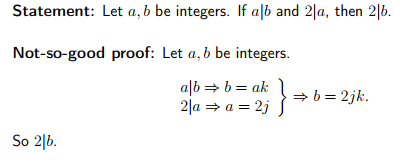
\includegraphics[scale = .75]{badproof.png}
	\end{figure}
\\
I would often forget to write out hypothesis and conclusions, even not defining new variables. After realizing these flaws in my proofs, I've been trying to improve my  formality. Its been a slow process but I believe I'm improving in comparison to the first few proofs we did in class.\\
\\
However, I think a strength I possess in academic writing is my step by step process to proving my proof. For example, in inductive proofs, I often forget my conclusion and problem statement, but I always believed my inductive hypothesis and inductive steps where always pretty solid.

\section{ Prove that the L$_{p}$ distance is a distance metric.}

Prove that the L$_{p}$ distance is a distance metric.\\
L$_{p} = d_{p}(x,y) = \Vert(x_{1} - y_{1})^{p} + (x_{2} - y_{2})^{p} \Vert^{\frac{1}{p}}$ \\
To be a distance metric, you must satisfy 4 requirements:\\
Let X = discrete space\\
A metric is a function d: X x X $\rightarrow$ $\R$ such that:
\begin{enumerate}
  \item d(x,y) = d(y,x)
  \item d(x,y) = 0 $\Leftrightarrow$ x = y
  \item d(x,y) + d(y,z) $\geq$ d(x,z)
  \item d(x,y) $\geq$ 0
\end{enumerate}
So,\\
Let $x,y$ in $\R^{n}$. Then $d(x,y) = max_{i} \Vert x_{i} - y_{i} \Vert$\\
Then $d(y,x) = max_{i} \Vert y_{i} - x_{i} \Vert$\\
$max_{i} \Vert x_{i} - y_{i} \Vert = max_{i} \Vert y_{i} - x_{i} \Vert$\\
Therefore $d(x,y) = d(y,x)$\\
\\
For all x,y in $\R$, Then $d(x,y) = max_{i} \Vert x_{i} - y_{i} \Vert$, therefore by definition of absolute value, the distance can never be negative.\\
Therefore, d(x,y) $\geq$ 0\\
\\
Given $d(x,z) = max_{i} \Vert x_{i} - z_{i} \Vert$\\ 
Then, $max_{i} \Vert x_{i} - z_{i} \Vert$ less than or equal to $max_{i} \Vert x_{i} - y_{i} + max_{i} \Vert y_{i} - z_{i} \Vert$ by the definition of the triangle inequality\\
Therefore, d(x,y) + d(y,z) $\geq$ d(x,z)\\
\\
For all $X = [x_{1}, x_{2}, ... x_{n}]$ and $Y = [y_{1}, y_{2}, ... y_{n}]$ in $\R$ if $max \Vert x_{i} - y_{i} \Vert$ = $min \Vert x_{i} - y_{i} \Vert$, then $X = Y$ for all $x_{i}$ in X and $y_{i}$ in Y. Therefore, if and only if X = Y then d(x,y) = 0\\
Therefore d(x,y) = 0 $\Leftrightarrow$ x = y\\
\\
L$_{p}$ fulfills all these conditions, therefore the L$_{p}$ distance is a metric distance.

\newpage
\section{Recall the randomized quicksort algorithm}

\subsection{Give pseudocode for a version of this algorithm that does not use recursion}

\begin{algorithm}
\caption{Iterative Quicksort}\label{euclid}
\begin{algorithmic}[1]
\State INPUT: Array
\State OUTPUT: Sorted Array
\State $new Stack$
\State $push(\$)$
\State $push(A.length() - 1)$
\While { $!Stack.isEmpty$}

\State head = pop()
\State tail = pop()
	\If {$tail - head \geq 3$} 
    \State $partition = head + ((tail - head)/2)$
    \State $partition = \bf{partition}(A, p, head, tail)$
    \\
    \State $push(partition + 1)$
    \State $push(tail)$
    \State $push(head)$
    \State $push(partition)$
    \EndIf
\EndWhile
\end{algorithmic}
\end{algorithm}

\subsection{Loop Invariant}
All elements less than head and greater than tail are smaller steadily increasing
$Referencing$ $https://en.wikibooks.org/wiki/Algorithm\_Implementation/Sorting/Quicksort$\\
\end{document}
